\chapter{Background}
\label{background}

\section{Introduction to Machine Learning}
In \textcite{MLANN}, Machine Learning is defined as "the question of how to
construct computer programs that automatically improve with experience".
Machine Learning has blossomed in recent years with applications across multiple
domains using vastly different paradigms and technologies.

There are many ways in which Machine Learning can be used in the modern world,
many of which are being utilised to great affect.
Some of these applications, are image recognition, natural language processing,
medical diagnosis and many more.
There may be fear that Machine Learning will start to take away many jobs from
humans but this may not be the case. Imagine a doctor, having to diagnose a
patient, a machine can offer suggestions based on very large datasets of what
the diagnosis is. This is not to say that a Machine would be
perscribing patients, but merely act as an assistant to the doctor.

Machine Ethics is a large problem that comes hand in hand with Machine Learning.
There is a very important question of who takes the blame when things go wrong,
that is why I think it is important that we only use Machine Learning to advise
and not to determine but this can be very difficult in a world where, for
example, an autonomous car has to decide between crashing into a vehicle beside
them with an unknown number of people inside or the two children playing in the
street.

One of the most exciting avenues in Machine Learning, in my opinion, is Computer
Vision. Computer Vision can be used in many areas to improve our lives. As
mentioned earlier, autonomous cars are only possible when a machine can
determine what objects are around it. Computer Vision can allow a machine to
recognise skin diseases in an image. The applications are nearly limitless and
that is without taking into account other uses.

\section{Machine Learning Paradigms}
There are many Machine Learning paradigms, all of which I will
discuss briefly below, but the main area of my focus for this project is in
Artificial Neural Networks (ANN). This is because I have researched extensively into Convolutional Neural Networks which are based on ANN's.
\subsection{Artificial Neural Networks}
An Artificial Neural Network is a bio-inspired system that is used to model the human brain in how it learns from experience.
The ANN uses this model to build a very complex web of connected units called
artificial neurons.
These nuerons are connected by certain weights which determines the processing
capacity of the network and these weights are created by learning a
dataset.(Malachy)
An ANN has a set of inputs that take in a value, sometimes from network outputs
and produce a single result or classification.
While an ANN is bio-inspired from the human brain, there are many elements of
the brain that are not present in ANN and many new elements in ANN that are not
modelled from the human brain.

Before I can talk about Convolution Neural Networks which are vital the image
processing, I will have to talk about the perceptron learning algorithm, the multi
layer percepton, and backpropogation.

\subsubsection{Perceptron Learning - Artificial Neuron}
In our Artificial Neural Network a Perecptron is an Artificial Neuron.
It is called an Artifical Neuron because it is a bio-inspired neuron which models
a neuron in the human brain in terms of inputs and output.

In Perceptron learning, we can take two inputs which are put towards an
activation function with a bias attached as seen in \ref{fig:perceptron}.
These inputs are multiplied by the weights that connect the input to the
activation function and depending on the result, the activation function may
fire an output.

\begin{figure}
     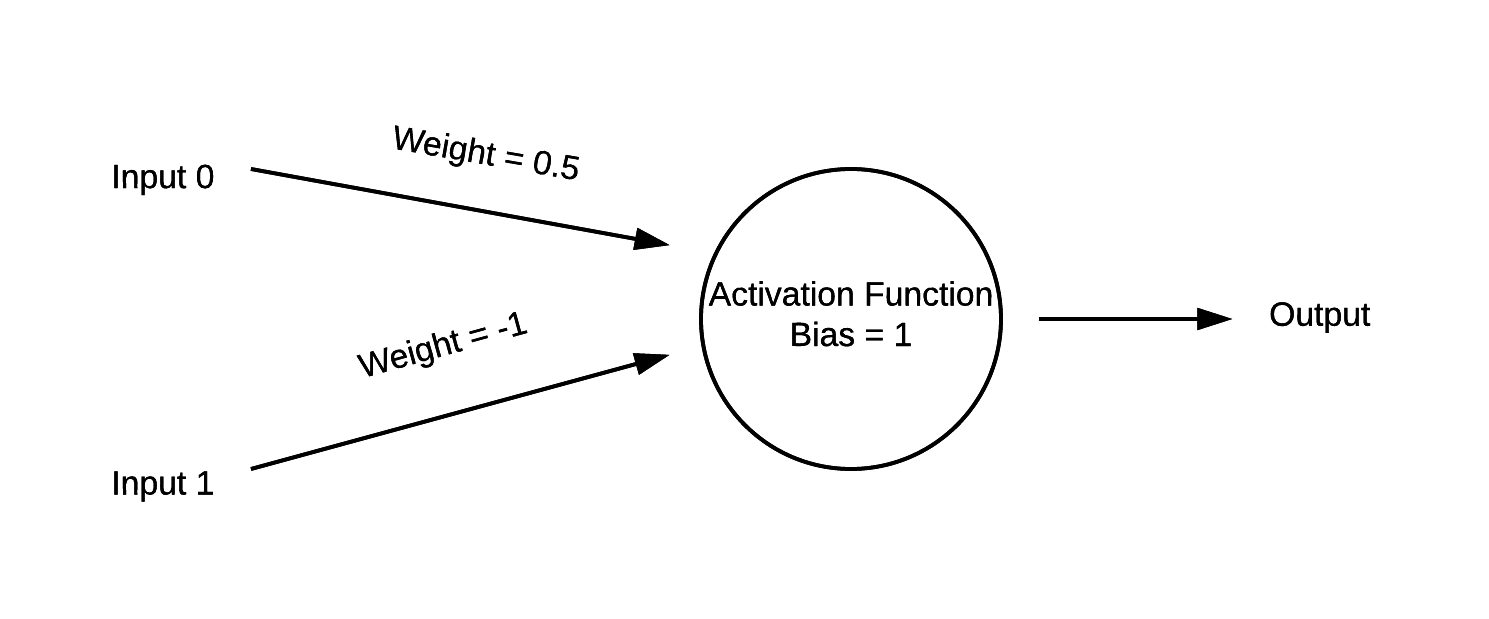
\includegraphics{Perceptron}
     \caption{Perceptron}
     \label{fig:perceptron}
\end{figure}

This Perceptron Learning Rule assumes that there are two sets of instances, a
positive and negative set, and each of these has an input and output domain.

\subsubsection{Multi Layered Perceptron}
Multi Layer Perceptrons (MLP) are made up of multiple layers of perceprons connected
together.
Firstly, we have an input layer, followed by one of more hidden layers and then
finally an output layer.
Any Neural Network with more than three hidden layers is categorised as a deep
layer.

Multi Layer Perceptrons are a class of feed forward Artificial Neural Networks.
These means that the output of each perceptron feeds into an input in the next
layer of the network.

\begin{figure}
    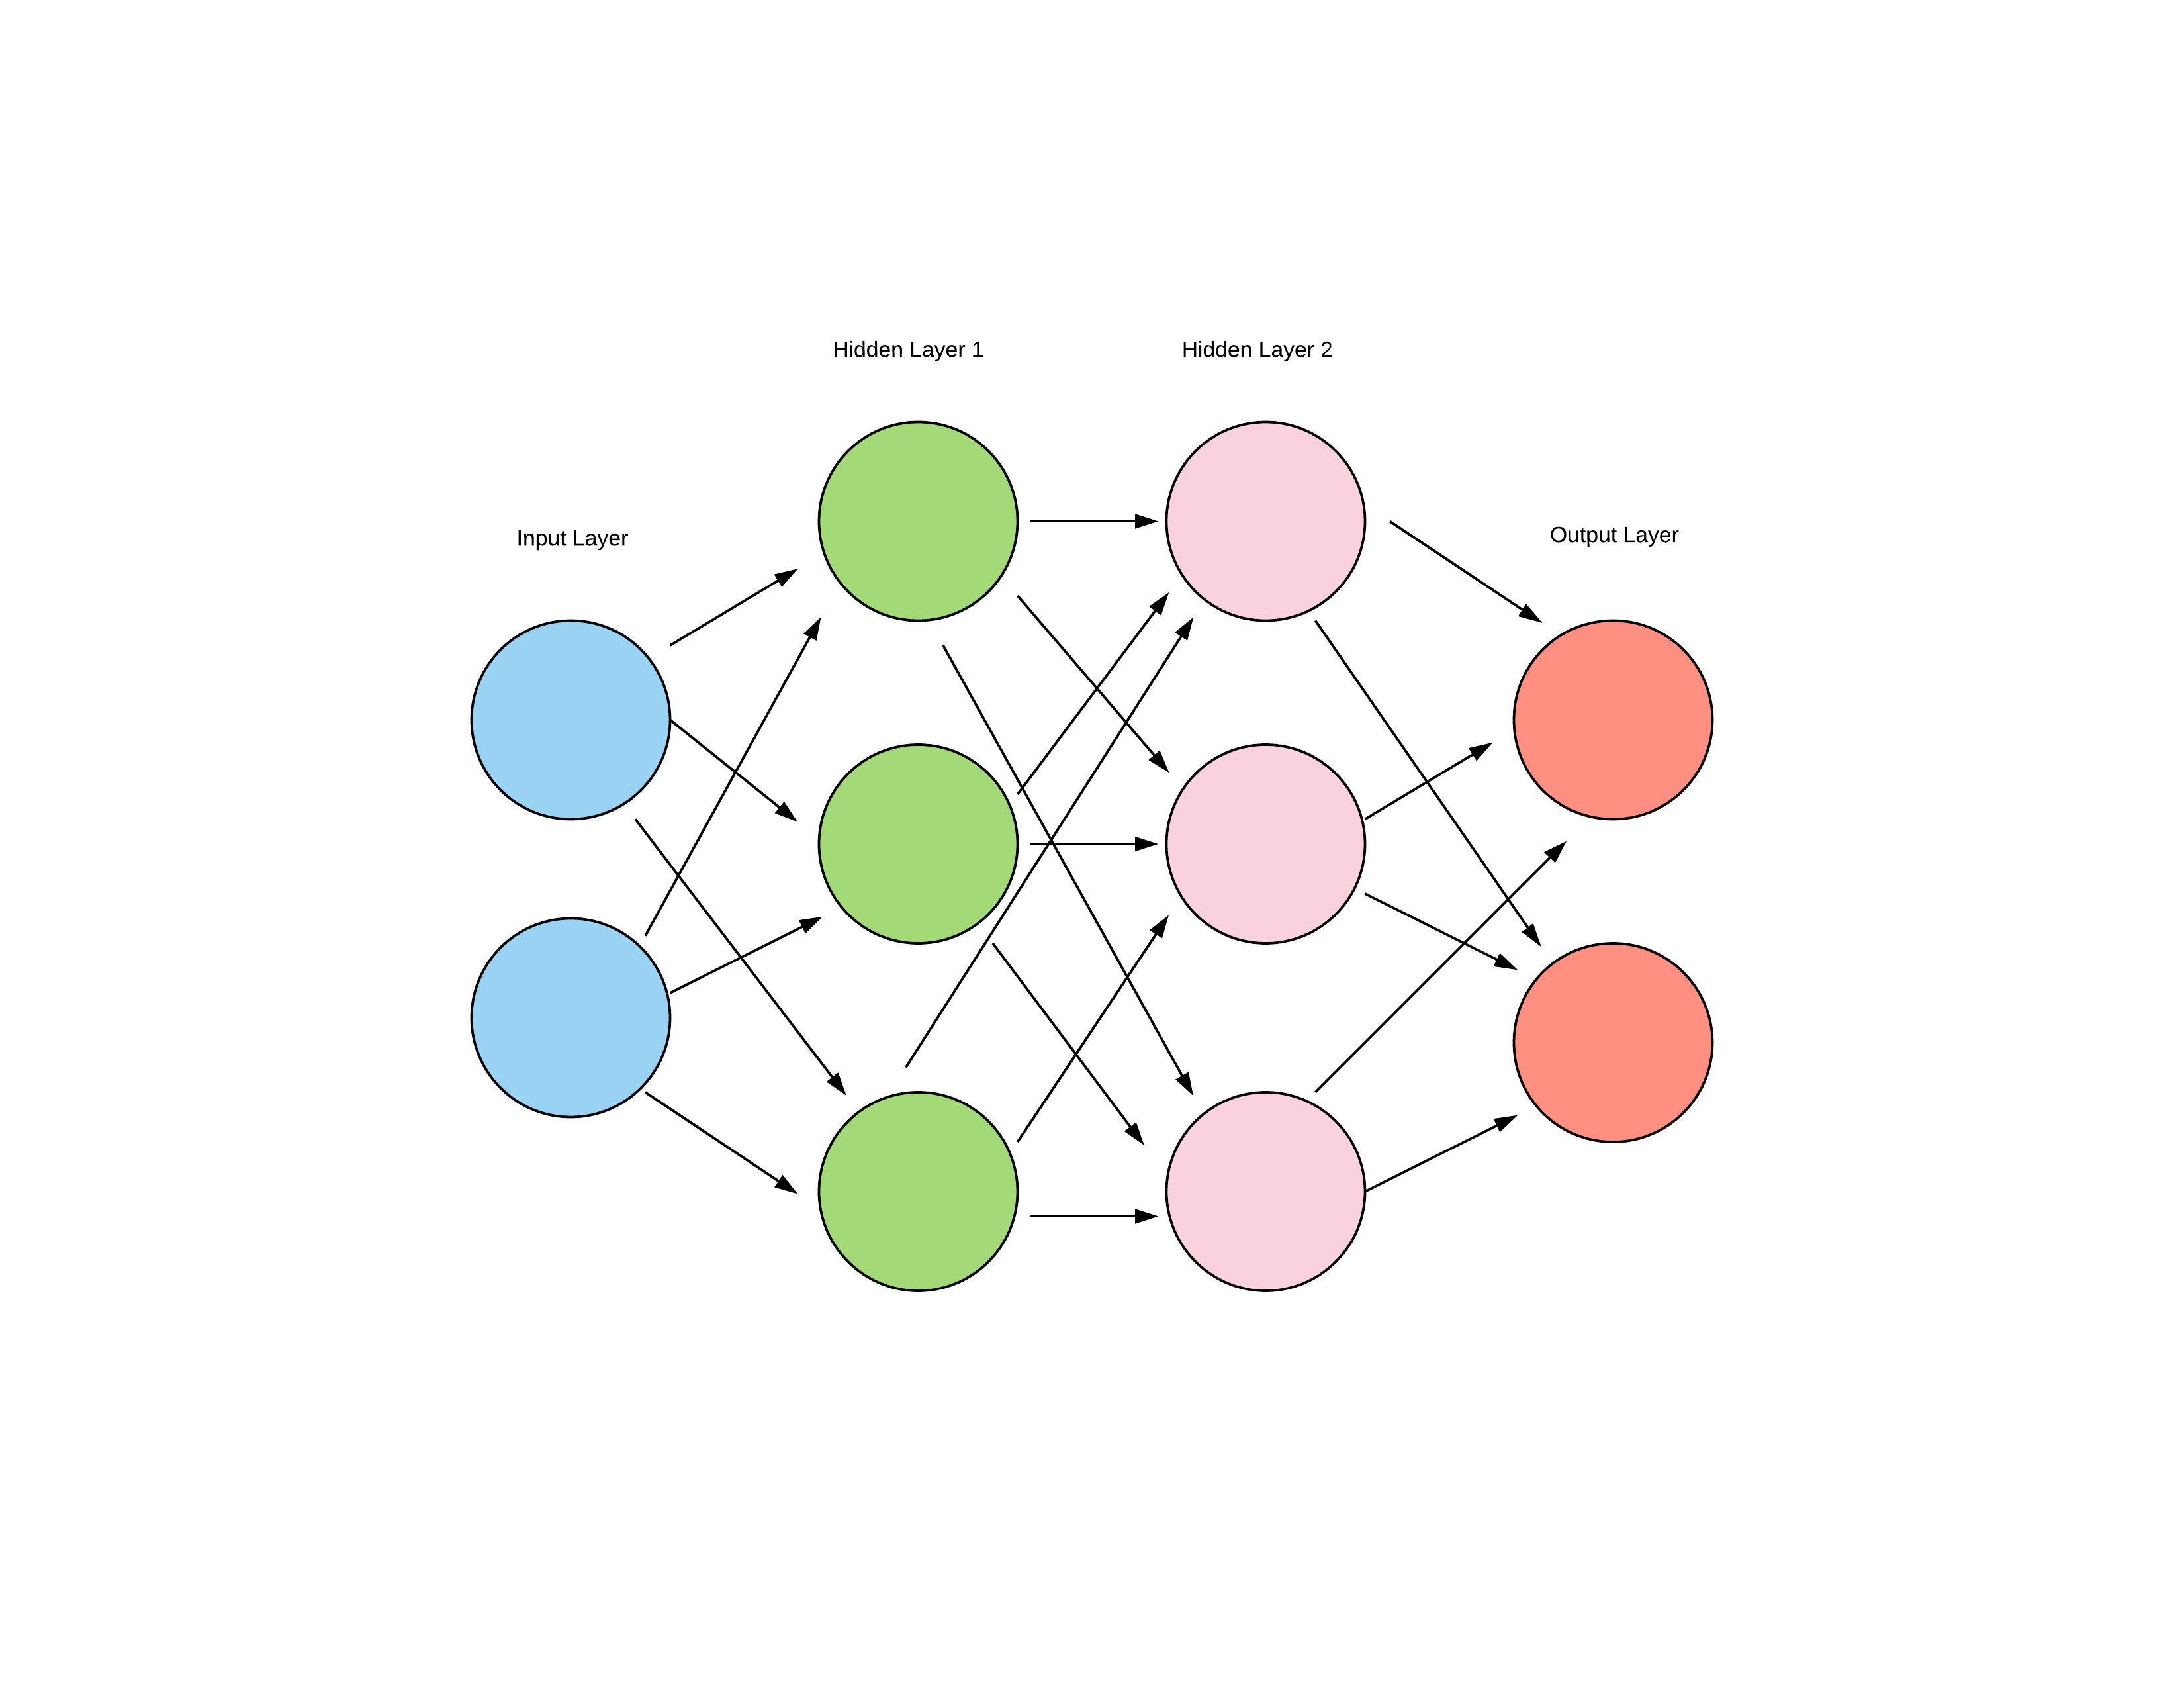
\includegraphics[width=150mm,scale=0.5]{mlp}
     \caption{Multi Layer Perceptron}
     \label{fig:mlp}
\end{figure}

\subsubsection{Gradient Descent and Backpropogation}
\tocless\subsubsection{Gradient Descent and backpropagation}
Gradient descent is an algorithm used to find the optimal weights to produce the
smallest prediction error. It is used to overcome problems of non-linearly
separable classes. Gradient descent search selects a random weight value and
then modifies it gradually to minimize the error. "At each step, the weight
vector is altered in the direction that produces the steepest descent along the
surface" \parencite{MLANN}. This step is iterated until the lowest value is met.

There is an error function used for the perceptron which finds the lowest error for that neuron, but it can't be used here because, since we have many neurons, there could be an error in multiple neurons.
Gradient descent is mathematically based on the derivative of a function.
The gradient of a function can be calculated by differentiating it.
As the weights are what is being controlled, "they are what we differentiate in respect to" \parencite{MLAlgorithm}.
The negative gradient of this function is followed to find the lowest possible point, hence the name gradient descent \parencite{MLAlgorithm}.

One problem with gradient descent is that if we look at Figure \ref{fig:GD}, we may
never get to the optimal point, point B. This is because we will find point A
without too many problems but when the weights change we will get too high a
slope of error and therefore will never reach point B.

Another variation of gradient descent is Stochastic Gradient Descent (SGD). SGD
is different because it updates "weights incrementally, following the
calculation of the error of each individual example" \parencite{MLANN}. 

\begin{figure}[h]
      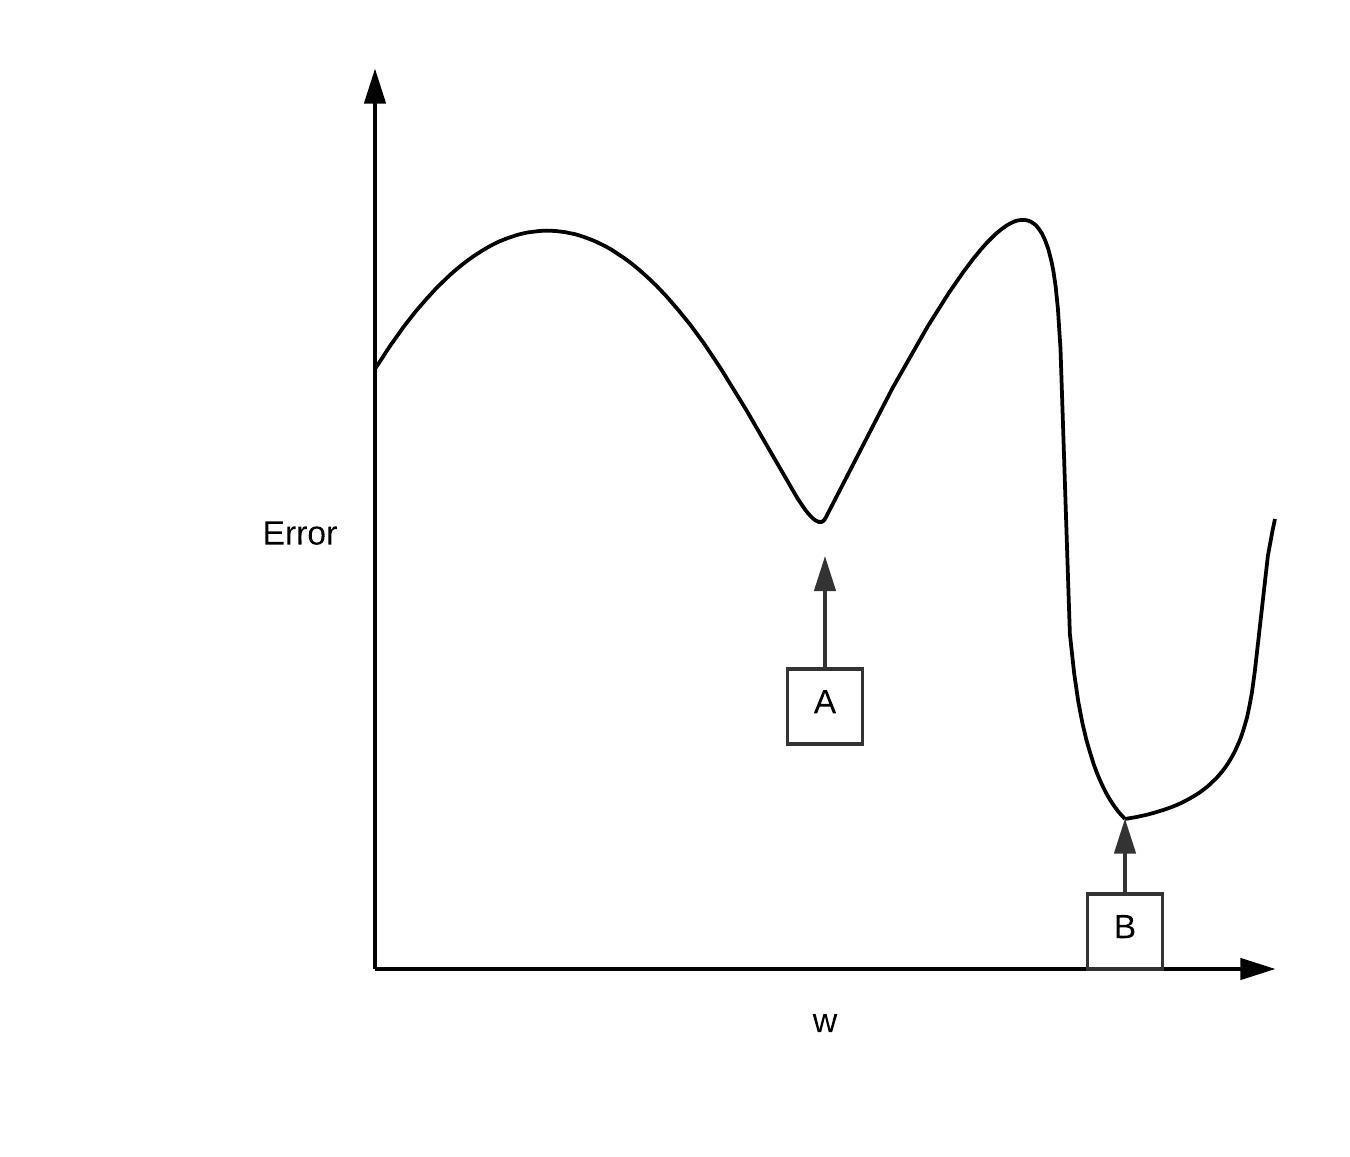
\includegraphics{GradientDescent}
      \caption{Gradient Descent}
      \label{fig:GD}
 \end{figure}

"The Backpropagation algorithm learns the weights of a multilayer network,
given a network with a fixed set of units and interconnections" \parencite{MLANN}.
Backpropagation attempts to minimize the mean squared error between the target
output and the actual output of a network.

Backpropagation works by starting at the output layer of the network and going
back through previous hidden layers, updating weights as it goes i.e. it propagates back through the network, updating the weights to try and reduce the error.

\parencite{MLANN} defined a walkthrough of the backpropagation algorithm.
For every value of Equation \ref{eqn:bp1}, in the training set where x is a vector of inputs and t is a vector of output values to act as a target:
\begin{itemize}
	\item{Run x through the network and output Equation \ref{eqn:bp2}.}
	\item{For each output k, calculate the error by Equation \ref{eqn:bp3}.}
	\item{For every hidden unit, calculate the error by Equation \ref{eqn:bp4}.}
	\item{Update weights by Equation \ref{eqn:bp5} where Equation \ref{eqn:bp5} is true.}
\end{itemize}

\begin{equation}\label{eqn:bp1}
    \vec{x}, \vec{t}
\end{equation}

\begin{equation}\label{eqn:bp2}
    o_{u}
\end{equation}

\begin{equation}\label{eqn:bp3}
    \delta_{k} \leftarrow o_{k}(1 - o_{k})(t_{k} - o_{k}) 
\end{equation}

\begin{equation}\label{eqn:bp4}
    \delta_{h} \leftarrow o_{h}(1 - o_{h}) \sum_{k \in outputs}   w_{kh}\delta_{k}
\end{equation}

\begin{equation}\label{eqn:bp5}
    w_{ji} \leftarrow w_{ji} + \Delta w_{ji}
\end{equation}

\begin{equation}\label{eqn:bp6}
    \Delta w_{ji} = \delta_{j} x_{ji}
\end{equation}


\subsubsection{Convolutional Neural Networks}
Convolutional Neural Networks (CNN's) are essentially a Multi Layered Percetron with a
special structure. CNN's have one major difference from a MLP, they have extra
layer of convolution and pooling.

Figure \ref{fig:XtoRec} show an image that we want to compare against
Figure \ref{fig:XtoComp}.
For humans, it is quite easy to determine that these images are very similar but
for a computer this task is surprisingly difficult.

So what a CNN does, to combat this problem, is to take a small feature from
Figure \ref{fig:XtoRec} and compare it to a subsection of Figure \ref{fig:XtoComp}.
The CNN multiplies the feature and a section of Figure \ref{fig:XtoComp}, adds
up the results and divides by 9. This then gives a decimal value of how likely
it is that the feature is in the part of the image, as seen in Figure
\ref{fig:convoluted}.
This is called filtering. The Convolutional layer is composed of carrying out
this filtering for every single possible location in Figure \ref{fig:XtoComp}.
\begin{figure}
      \begin{subfigure}[b]{0.4\textwidth}
          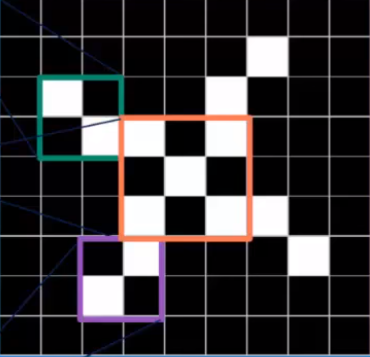
\includegraphics[width=\textwidth]{XtoRec}
          \caption{Image to Classify}
          \label{XtoRec}
      \end{subfigure}
    %
      \begin{subfigure}[b]{0.4\textwidth}
      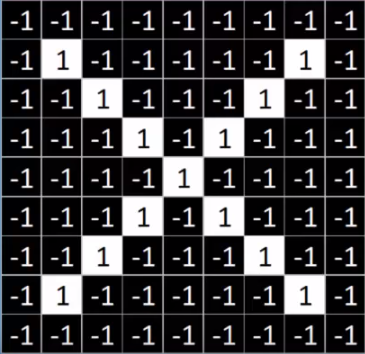
\includegraphics[width=\textwidth]{XtoComp}
      \caption{Image to Compare}
      \label{XtoComp}
      \end{subfigure}
\end{figure}

\begin{figure}
      \begin{subfigure}[b]{0.4\textwidth}
          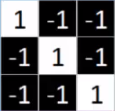
\includegraphics[width=\textwidth]{ImageFeature}
          \caption{Image Feature to Search}
          \label{fig:feature}
      \end{subfigure}
     %
      \begin{subfigure}[b]{0.4\textwidth}
           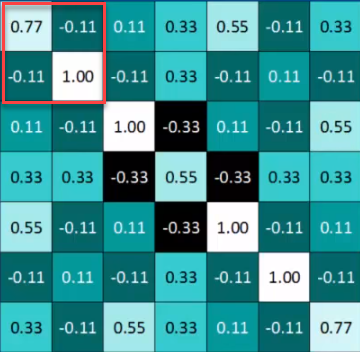
\includegraphics[width=\textwidth]{ConvImage}
           \caption{Convoluted Image}
           \label{fig:convoluted}
      \end{subfigure}
\end{figure}
\begin{figure}
    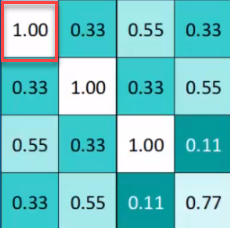
\includegraphics[width=50mm,scale=0.5]{PooledImage}
    \caption{Pooled Image}
    \label{fig:pooled}
\end{figure}
Next is the Pooling Layer, what this layer does, is it takes the convoluted
layer output, you can use Figure \ref{fig:convoluted} as reference, and from a
user defined size ie. 2x2, gets either the highest decimal value (Max pooling)
or the average value (Mean pooling) and records that as the new value for the
section. This is then applied to the entire image. As we can see in Figure
\ref{fig:pooled} we know have a much smaller image stack in which to classify,
thus making the computation easier.

In between the Convolution and Pooling layer, there is sometimes a Normalization
layer. This Normalization layer creates Rectified Linear Units (RLU's). In other
words, if we take Figure \ref{fig:convoluted}, it changes all minus values to
zero.

\subsubsection{Fully Convolutional Networks}
A Fully Convolutional Network is one that does not have a fully connected layer
and in a fully connected layers place is another convolution layer.

\subsection{Other Paradigms}
There are many other Machine Learning paradigms apart from Neural Networks, each of which I will give a brief
introduction.

\subsubsection{Decision Trees}
"Decision tree learning is  method for approcimating disrete-valued target
functions, in which the learned function is represented by a descision tree"
\textcite{MLDT}. There are many different classification algorithms that can
create decision trees from supervised learning.

\subsubsection{Bayesian Learning}
\subsubsection{Instance Based Learning}
\subsubsection{Logistic Regression}
\subsubsection{Support Vector Machine}
\subsubsection{Regression Analysis}
\subsubsection{Unsupervised Learning}
\subsubsection{Reinforcement Learning}

\section{Overview of Machine Vision Approaches to Identification and Classification}
There have been many attempts of identification and classification by many
different researchers over the last number of years. There some approaches that
decouple the two tasks of identification and classification from one another but
mostly, researchers have attempted the two together. Sometimes, by semantic
segmentation and in others simply building a classifier for the image without
taking into account, the need for object identification.

\subsection{Region Based Convolutional Neural Networks}
Due to the issues with composite images (images with multiple items) in food image recognition, an object detection approach may prove to be successful.
If the objects (different food items) in an image could be classified seperately then the overall effiency of a nutrional assessment system, aided by deep learning, could be improved.
Ross Girshik and other contributors had some very positive results in the area
of object detection using region based convolutional neural networks. There were
four iterations of papers based on this work by Ross and groups in UC Berkley,
Microsoft and Facebook. A PHD student at the time of Ross's first paper also
completed his dissertation on the subject. These papers, their
results (Table \ref{rcnnResults}) and the changes made through each iteration will be analysed thoroughly in the proceeding sections.

In the first paper written by Ross Girshik, while researching at UC Berkeley,
focused on two main insights. These were that " one can apply high-capacity convolutional neural networks (CNNs) to bottom-up region proposals in order to localize and segment objects" and that
"when training data is scarce, supervised pre-training for n auxiliary task,
followed by domain-specific fine-tuning, yields a significant performance boost"
\parencite{rcnn}.

The system that they developed followed these steps:
\begin{itemize}
    \item{Take image as input}
    \item{Extract approximately 2000 region proposals from the image}
    \item{Compute fixed length vectors of features for the regions using a convolutional
        neural network}
    \item{Use a Support Vector Machine (SVM) to classify these regions}
    \item{Bounding box regression for final region proposals}
\end{itemize}

This system utilised selective search to gather these region proposals, but they
mention that a sliding-window detector is also an option. Ross Girshik and his
team used the open source Caffe CNN library for this system. The system is quite
efficient and scalable. It is scalable because of the fixed length vector of
features which will remain constant regardless of inputs and additional outputs.
The team evaluated their results on a few metrics and test sets as seen in Table
\ref{rcnnResults}. Explanation of the datasets used can be seen in Table \ref{datasets}.

Ross Girshik's next iteration of work on region based convolution neural
networks took place in Microsoft Research. This paper was titled "Fast R-CNN" as
its aim was to decrease training and testing time "while also increasing
detection accuracy" \parencite{fastRcnn}.

This paper analyses why RCNN \parencite{rcnn} was slow and therefore how it could be improved.
RCNN was classified to be slow because of three main factors:
\begin{itemize}
	\item{There are multiple stages to training as both a CNN and a SVM need to
		be trained.}
	\item{In training of the SVM, each region proposal must be written to disk
		and is therefore expensive.}
	\item{Object detection takes 47 seconds per image}
\end{itemize}

Due to these problems with RCNN, a new algorithm, titled Fast RCNN was proposed.
The architecture is as follows. An image is taken as input along with a
proposal for regions. The image is pushed through convolutional and pooling
layers (using max pooling). A fixed-length vector of features is then extracted
from each region proposal. These vectors are inputted to fully connected
layers for bounding box location prediction.
At detection time, a pass through of the net is all that is needed so this
runtime is significantly less than RCNN.

Due to the success of RCNN and Fast RCNN, Faster RCNN was introduced to combat
the problem of region proposal computation \parencite{fasterRcnn}.
The architecture for this system comprises of two modules. These consist of a
convolutional neural network for region proposals (RPN) which the feeds into a Fast
RCNN detector. These combine to produce a single neural network for object
detection.

Instead of training these networks separately, the team had to look at how to
share layers between the two networks. There were three options available:
\begin{itemize}
    \item{Alternating training whereby RPN is trained, and then used to train
        Fast RCNN. The Fast RCNN network is then used to initialise RPN and the
		process is iterated \parencite{fasterRcnn}. This paper follows this approach.}
    \item{Approximate joint training.}
    \item{Non- approximate joint training.}
\end{itemize}

\begin{table}[h]
    \centering
    \caption{Results from Region Based CNN Research}
    \label{rcnnResults}
    \begin{tabular}{|p{1.5cm}|l|l|l|l|l|l|}
    \hline
                    & \textbf{VOC07} & \textbf{VOC10} & \textbf{VOC11} & \textbf{VOC12} & \textbf{COCO15} &
                    \textbf{COCO16} \\ \hline
                    RCNN        & 58.5\%  & 53.7\%  & 47.9\%  & N/A     & N/A
                    & N/A      \\ \hline
                    Fast RCNN   & 70.0\%  & 68.8\%  & N/A     & 68.4\%  & N/A
                    & N/A      \\ \hline
                    Faster RCNN & 78.8\%  & N/A     & N/A     & 75.9\%  & 42.7\%
                    & N/A      \\ \hline
                    Mask RCNN   & N/A     & N/A     & N/A     & N/A     & N/A
                    & 63.1\%  \\ \hline
    \end{tabular}
\end{table}

\begin{table}[h]
\centering
\caption{Datasets}
\label{datasets}
\begin{tabular}{|p{1.65cm}|p{10.5cm}|}
\hline
\textbf{Table} & \textbf{Explanation}                                                                                                                                                                                               \\ \hline
VOC07          & The PASCAL VOC dataset is used for the PASCAL (Pattern Analysis, Statistical Modelling and Computational Learning) Visual Object Classes Challenge. \parencite{pascal-voc-2007} was used for the 2007 challenge. \\ \hline
VOC10          & The PASCAL VOC 2010 dataset was used for the 2010 challenge \parencite{pascal-voc-2010}.                                                                                                                         \\ \hline
VOC11          & The PASCAL VOC 2011 dataset was used for the 2011 challenge \parencite{pascal-voc-2011}.                                                                                                                        \\ \hline
VOC12          & The PASCAL VOC 2012 dataset was used for the 2012 challenge \parencite{pascal-voc-2012}.                                                                                                                        \\ \hline
COCO15         & The COCO (Common Objects in Context) dataset created by Microsoft (\parencite{coco}) is used to measure the efficacy of object detection algorithms. The COCO 2015 dataset was released in 2015 for training.    \\ \hline
COCO16         & An updated version of the COCO dataset was released in 2015.                                                                                                                                                       \\ \hline
\end{tabular}
\end{table}

The most recent paper on this topic was also written by Ross Girshik while
working with Facebook AI Research \parencite{maskRcnn}. Mask RCNN " extends Faster
RCNN by adding a branch for predicting an object mask in parallel with the
existing branch for bounding box regression" \parencite{maskRcnn}.
Mask RCNN has two modules, like Faster RCNN, where the first module is the
Region Proposal Network. In the second module, in parallel to classification, a
binary mask is outputted for each region. Bounding box regression and
classification are done in parallel.


\subsection{Fully Convolutional Neural Networks for Semantic Segmentation}
There has been a very interesting paper from UC Berkeley focused on using Full Convolutional
Networks for semantic segmentation \parencite{fcn}. Fully Convolutional Networks
(FCN)
do not have any fully connected layers. They are replaced with more filtering
layers. Nvidia Digits have a semantic segmentation implementation based off the
work of this paper.

They took this approach because "feedforward computation and backpropogation are
much more efficient when computer layer-by-layer over an entire image instead of
independently patch-by-patch" \parencite{fcn}. This was also because they
were focused on object detection. Normal classifiers do not work very well when
they are to classify more than one subject in an image and image segmentation
was a way to solve this.

There are a set of steps you can follow to turn a CNN into a FCN for semantic
segmentation as follows ie. change to a convolutional layer from a fully
connected one:
\begin{itemize}
    \item{The size of the filters must be set to the size of the input layers.}
    \item{For every neuron in the fully connected layer, have a filter.}
\end{itemize}

\begin{table}[]
\centering
\caption{FCN Resulys \parencite{fcn}}
\label{fcn}
\begin{tabular}{ll}
                        & FCN  \\
VOC11 mean IU           & 62.7 \\
VOC12 mean IU           & 62.2 \\
PASCAL VOC10 pixel acc. & 67.0 \\
PASCAL VOC10 mean acc.  & 50.7 \\
PASCAL VOC10 mean IU    & 37.8 \\
PASCAL VOC10 f.w. IU    & 52.5
\end{tabular}
\end{table}

\subsection{Image Segmentation}
\subsubsection*{Graph Based Segmentation}
Graph cut segmentation has been used extensively  in image segmentation. OpenCV
has an implementation of a graph cut algorithm called grabcut which has been
used to segment food on occasion \textcite{graphCut}. 

According to \textcite{graphCut}, "Graph cut based method is well-known to be
efficient, robust, and capable of finding the best contour of objects in n
image, suggesting it to be a good method for separating food portions in a food
image for calorie measurement". Along with the graph cut segmentation algorithm,
this research team also used color and texture segmentation. Gabor filters were
used to measure texture features \textcite{graphCut}. When color and texture
segmentation was applied, the method came into difficulty with mixed foods but
by applying graph cut segmentation, clearer object boundaries were shown.

In conclusion, the accuracy of the classification increased when using graph
based segmentation rather than color and texture as seen in \ref{graphCT}.

\begin{table}[]
	\centering
	\caption{Results}
	\label{graphCT}
	\begin{tabular}{llll}
		                  & Single Food Portion & Non-mixed Food & Mixed Food
						  \\
						  Color and Texture & 92.21               & N/A
						  & N/A           \\
						  Graph Based       & 95 (3\% increase)   & 5\% increase
						  & 15\% increase
	\end{tabular}
\end{table}

\subsubsection*{Local Variation Framework}
Another paper was published in which the research team attempted to create a
food calorie extimation system \textcite{foodImageAnalysis}. This system would
compromise of three steps, image segmentation, image classification and weight
estimation. For the segmentation module, a local variation approach to
segmentation was performed. Local variation is by which intensity differences
between neighbouring pixels is measured. This is a type of graph based
segmentation.

The team also carried out some segmentation refinement when the segmentation
algorithm had been performed. This consisted of removed small segments (defined
as less than 50 pixels) and trying to prevent over and under segmentation. After
classification was performed on each segment, segments with low confidence
values were removed \textcite{foodImageAnalysis}.

\subsubsection*{Conclusion}
Both of the above papers of \textcite{graphCut} and \textcite{foodImageAnalysis}
used a graph based segmentation. The first paper used a more generic
implementation while the second used a local variation framework. Both methods
provided successful results in the image segmentation process.

\subsection{Convolutional Neural Networks for Classification}
Many researchers have used convolutional neural networks for image
classification with various network architectures and many have used a food image dataset.
Some of these papers will be looked at below.
A summary of their results can be seen in Table \ref{cnn_summary}.

\parencite{deepLearning} focused on a deep learning approach to food image recognition based
their neural network architecture on Inception-ResNet and Inception V3.
Deep learning is a term usually given to algorithms based on neural networks.
They also used the Food-101 dataset. For this system, Google's
Tensorflow was used for image preprocessing. Preprocessing was needed as the
environmental background is different in many food images. Because of these
"Grey World method and Histogram equalization" \parencite{deepLearning} were
used.
Amazon Web Services (AWS) Graphics Processing Units (GPU) instances were used for training.
AWS instances are cloud servers.
The results on completion were quite impressive with a Top-1 Accuracy of 72.55\% and a Top-5 Accuracy of 91.31\%.

Another research team in Japan, \parencite{yanaiFood} researched this topic. This was built off previous research they had carried out in the field \parencite{kawano2014food}.
They were aware of how
difficult the problem was and therefore employed many techniques to solve the
problem such as "pre-training with the large-scale ImageNet data, fine-tuning
and activation features extracted from the pre-trained DCNN". 
In conclusion, they found that the "fine-tuned DCNN which was pre-trained
with 2000 categories" from ImageNet was the best method. A
DCNN is a Deep Convolution Neural Network. 
A network can become a DCNN when the number of hidden layers is larger than three.
While many of the CNNs discussed have been DCNN, most are just labeled as CNNs.
The achieved results of 78.77\% for Top-1 Accuracy in the UECFOOD100 dataset.


\parencite{kagayaFood} also employed the use of convolutional neural networks for
image detection. They used a CNN for the "tasks of food detection and recognition
through parameter optimization".
They found that a CNN is much better suited to the task than a Support Vector
Machine (SVM). They achieved an overall classification accuracy of 93.8\%
against their baseline accuracy of 89.7\%. This accuracy
was calculated using a dataset that they created specifically for this task.
When they had completed the task they analysed the trained convolutional kernels
and came to an interesting conclusion. They found that "color features are
essential to food image recognition".


The last paper that will be analysed, \parencite{deepFood}, oriented around using a Convolutional Neural
Network for food image recognition, focuses on developing a dietary assessment
application for use on a smart phone. They used the UEC-256 and Food-101 dataset
for their experiments and achieved impressive results.
They used a Convolutional Neural Network but "with a few major optimizations,
such as optimized model and an optimized convolution technique". 
They used the Inception module for their CNN. After the
inception module was complete, they made the GoogleNet architecture by combining modules. In
total, the network had 22 layers.
They achieved the results shown in Table \ref{resultsDeepFood}.

\begin{table}[h]
	\centering
	\caption{DeepFood Results}
	\label{resultsDeepFood}
	\begin{tabular}{lll}
		& Top-1  & Top-5  \\
		UEC-256                   & 54.7\% & 81.5\% \\
		UEC-100                   & 76.3\% & 94.6\% \\
		Food-101                  & 77.4\% & 93.7\% \\
		UEC-256 With Bounding Box & 63.8\% & 87.2\% \\
		  UEC-100 With Bounding Box & 77.2\% & 94.8\%
	\end{tabular}
\end{table}

\parencite{nutrinet} developed a new neural architecture specifically for detecting food and drink images using deep convolutional neural networks called NutriNet.
The trained network was to be used to aid patients with Parkinson's disease in monitoring their diet.
NutriNet was created based off of the AlexNet architecture.
The dataset used for this study consisted of approximately 500 images for each of over 500 classes.
Through this dataset a Top-1 accuracy of 86.72\& and a Top-5 accuracy of 94.47\% was recorded.
A smart phone application was used for real world testing which brought a Top-5 accuracy of 55\%.
The application also saved these real world images from the smart phone to increase their dataset size.
In conclusion, the team found that there were modifications that could be made to the NutriNet architecture as real world images didn't perform incredibly well due to occlusion and background noise in the images.
The detection and recognition steps were separated in this architecture.
The team also acknowledges that joining these steps into a single DCNN may be successful and should be explored.

\begin{table}[h]
	\centering
	\caption{Summary of results in CNN based methods}
	\label{cnn_summary}
	\begin{tabular}{lll}
		Title                                & Dataset     & Top-1 Accuracy \\
		\parencite{deepLearning} 			 & Food 101    & 72.55\%  \\
		\parencite{yanaiFood}               	 & UECFood101  & 78.77\%  \\
		\parencite{kagayaFood}       		 & Own dataset & 93.80\%   \\
		\parencite{deepFood}                  & Food 101    & 77.40\%  	\\
		\parencite{nutrinet}                  & Own dataset & 86.72\%
	\end{tabular}
\end{table}



\section{Technologies}
\subsection{Tensorflow}
TensorFlow is a deep learning software library for various machine learning paradigms. TensorFlow will be used to create neural networks.
TensorFlow uses a data structure called a tensor which is basically an array of n dimensions.
TensorFlow has two utilisations, through a Graphics Processing Unit (GPU) and through a Central Processing Unit (CPU).
GPU computation is recommended for CNN training. 

\tocless\subsubsection{Central Processing Unit Computation}
It is quite easy to get TensorFlow up and running if you are only using a CPU to
train. TensorFlow CPU has been successfully installed on both Windows and Ubuntu, for this project.
For Windows you can download and install using the TensorFlow website and on ubuntu you can
using apt-get. Once installed, TensorFlow can be imported into any python shell
or script for use. TensorFlow can also be used in C++. There will be various
python implementations of neural networks in Chapter 3.

\tocless\subsubsection{Graphics Processing Unit Computation}
For use with a GPU, the set up for TensorFlow is a bit more complicated. Firstly
you must check that the GPU in your machine is compatible for CUDA 8.0 using the
NVIDIA website. If your GPU is compatible, you must install CUDA after signing
up as an NVIDIA developer. CUDA 8.0 is compatible with TensorFlow.
You also need to install cudnn6.
The NVIDIA website contains tutorials to install these.
Once these are installed, download and install tensorflow-gpu.
This can be imported into python similar to CPU computation.

\subsection{Jupyter}
\input{tex/tech/jupyter}
\subsection{OpenCV}
OpenCV is an industry wide, open source library for computer vision and machine learning \parencite{opencv}.
It has over 2500 algorithms that are available for use \parencite{opencv}.
OpenCV is supported across multiple languages and platforms such as Python, C++, C, Java, Matlab, running on Windows, Android, Mac OS and Linux \parencite{opencv}.

There is not much of the library utilised in this project due to the nature of Tensorflow but some algorithms for image reading, writing and resizing were used due to the ease of use.

\begin{lstlisting}
image = cv2.imread('image.jpg')
\end{lstlisting}

\begin{lstlisting}
resized = cv2.resize(image, (299, 299))
\end{lstlisting}

\begin{lstlisting}
cv2.imwrite('imageResized.jpg', resized)
\end{lstlisting}


\section{Evaluating the Output}
There are various different metrics that can be used for evaluating the output
of a classifier or segmentation algorithm, many of which we have seen in previous
sections. I was analyse a few of these evaluations of results so that I can use
them as a reference to apply to my own experiments. I will also look into some
problems associated with evaluating models.

\subsection{Research into Diagnosing Errors in Object Detectors}
There has been some research into the question of how to evaluate object
detectors, one of which I will discuss in detail \textcite{diagnosingErrors}.
This paper in question "analyzes the influences of object characteristics on
detection performance and the frequency and impact of different types of false
positives" \textcite{diagnosingErrors}. They found that there were many effects
that had influence on detectors as follows:
\begin{itemize}
    \item{occlusion}
    \item{size}
    \item{aspect ratio}
    \item{visibility of parts}
    \item{viewpoint}
    \item{localization error}
    \item{confusion with semantically similar objects}
    \item{confusion with other labeled objects}
    \item{confusion with background}
\end{itemize}

The research team goes on to analyse false positives in object detectors.
Localization errors were a large factor. This is were bounding boxes overlap to
other objects in the image. Confusion with similar objects had a large influence
on false positives also by which, for example, a dog detector had a high score
for a cat \textcite{diagnosingErrors}. Confusion with dissimilar objects and
confusion with background are the categories of the rest of the false positives
they measured.

In conclusion the team would that "Most false positives are due to misaligned
detection windows or confusion with similar objects"
\textcite{diagnosingErrors}. They had some recommendations towards improves
detectors as follows:
\begin{itemize}
	\item{Smaller objects are less likely to be detected}
	\item{Localization could be improved}
	\item{Reduce confusion with similar categories}
	\item{Robustness to object variation}
	\item{More detailed analysis}
\subsection{Detection Average Precision}
See \ref{fig:dap}.
\begin{figure}
	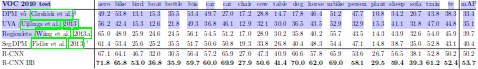
\includegraphics[width=150mm,scale=0.5]{DAP}
	\caption{Detection Average Precision \textcite{donahue}}
    \label{fig:dap}
\end{figure}

\subsection{Mean Average Precision}
See \ref{fig:MAP}.
		\begin{figure}
			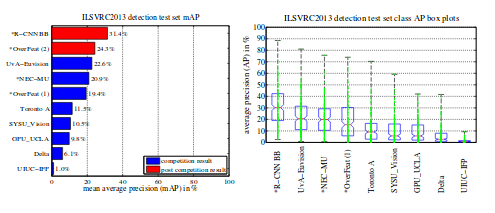
\includegraphics[width=150mm,scale=0.5]{MAP}
			\caption{Mean Average Precision \textcite{donahue}}
			\label{fig:MAP}
		\end{figure}
		
\subsection{Distribution of top-ranked false positives}
See \ref{fig:DFP}.
		\begin{figure}
			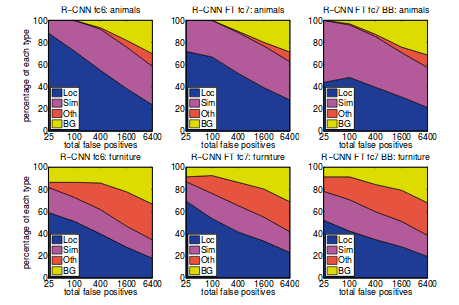
\includegraphics[width=150mm,scale=0.5]{DFP}
			\caption{Distribution of top-ranked false positives \textcite{donahue}}
			\label{fig:DFP}
		\end{figure}
		

\subsection{Segmentation Mean Accuracy}
See \ref{fig:SMP}.
		\begin{figure}
			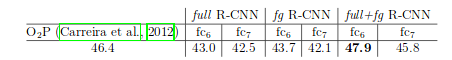
\includegraphics[width=150mm,scale=0.5]{SMP}
			\caption{Segmentation Mean Accuracy \textcite{donahue}}
			\label{fig:SMP}
		\end{figure}
		

\subsection{Per-category segmentation accuracy}
See \ref{fig:PCATSA}.
		\begin{figure}
			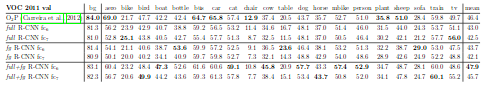
\includegraphics[width=150mm,scale=0.5]{PCATSA}
			\caption{Per-category segmentation accuracy \textcite{donahue}}
			\label{fig:PCATSA}
		\end{figure}
		

\subsection{Per-class segmentation accuracy}
\See \ref{fig:PCLASSA}.
		\begin{figure}
			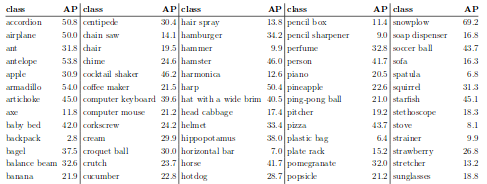
\includegraphics[width=150mm,scale=0.5]{PCLASSSA}
			\caption{Per-class segmentation accuracy \textcite{donahue}}
			\label{fig:PCLASSA}
		\end{figure}
		



